
\documentclass[fleqn,10pt]{wlscirep}

\usepackage{chemformula}
\usepackage{amsmath}

\title{Stochastic Dynamics of RNA interference: A Single-Molecule Time-based Approach}

\author[1*]{Baihan Lin}
\affil[1]{Department of Applied Mathematics, University of Washington, Seattle, WA 98195, USA}
\affil[*]{doerlbh@gmail.com}

\keywords{RNA interference, Central dogma, Stochastic gene expression, Chemical master equation, Single molecule}

\begin{abstract}

Under a general mechanistic understanding of RNA interference, we present a stochastic model for the cellular dynamics of gene expression involved in RNA interference in a single-molecule time-based approach.

\end{abstract}
\begin{document}

\flushbottom
\maketitle
%\thispagestyle{empty}

\section*{Introduction}

\cite{Figueredo:2009dg} 

As shown in Figure \ref{fig:diagram}, the RNA interference can be simplified as a genetic circuit, where central dogma determines that one set of DNA was transcribed into messenger RNA (mRNA) and interfering RNA (iRNA), mRNA were translated to protein, while iRNA inhibit the translation of mRNA.

\begin{figure}[ht]
\centering
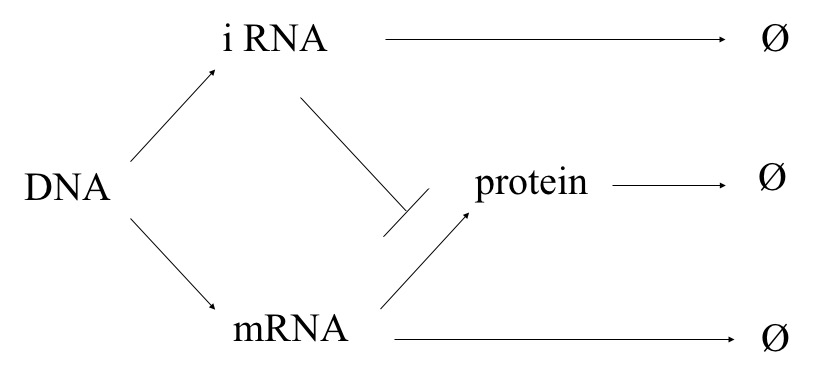
\includegraphics[width=6cm]{diagram}
\caption{a diagram for the genetic circuit simplification of RNA interference}
\label{fig:diagram}
\end{figure}


\section*{Results}

To simply the model, I used iRNA to represent microRNA and siRNA, which are similar RNA interference agents. Below is the proposed model on gene expression. Instead of producing transcription factor to bind with DNA, iRNA tends to bind with mRNA and form a complex to inhibit the translation. I made several assumptions, including same degradation rate for iRNA and mRNA, irreversible inhibition f = 0, etc..
 
The chemical reactions involved in this process is therefore summarized as these      steps:

\begin{itemize}
\item \ch{DNA + NTPs ->[k1] DNA + mRNA}
\item \ch{DNA + NTPs ->[k2] DNA + iRNA}
\item \ch{mRNA + AAs ->[k3] mRNA + protein}
\item \ch{mRNA + iRNA + RISC <=> [h][f] mRNA.iRNA.RISC}
\item \ch{mRNA ->[$\gamma$1] $\emptyset$}
\item \ch{iRNA ->[$\gamma$1] $\emptyset$}
\item \ch{mRNA.iRNA.RISC ->[$\gamma$2] $\emptyset$}
\item \ch{protein ->[$\gamma$3] $\emptyset$}
\end{itemize}
 
\subsection*{Deterministic Dynamics and Nonequilibrium Steady States}

Based on above reactions, following the law of mass action, the ordinary differential equation can be written:

\begin{equation}
\frac{d[iRNA]}{dt} = k_2[DNA][NTPs] - \gamma_1[iRNA] + f[mRNA.iRNA.RISC] - h[RISCs][iRNA][mRNA] 
\end{equation}
\begin{equation}
\frac{d[mRNA]}{dt} = k_1[DNA][NTPs] - \gamma_1[mRNA] + f[mRNA.iRNA.RISC] - h[RISCs][iRNA][mRNA]  
\end{equation}
\begin{equation}
\frac{d[mRNA.iRNA.RISC]}{dt} = (- f - \gamma_2)[mRNA.iRNA.RISC] + h[RISCs][iRNA][mRNA] 
\end{equation}
\begin{equation}
\frac{d[protein]}{dt} = k_3[mRNA][NTPs] - \gamma_3[protein]
\end{equation}

Since the concentrations of DNA, AAs, NTPs, RISCs can be considered to be maintained in the cell, we can simplify the system by denoting:

\begin{equation}
K_1 = k_1[mRNA][NTPs]
\end{equation}
\begin{equation}
K_2 = k_2[mRNA][NTPs]
\end{equation}
\begin{equation}
K_3 = k_3[AAs]
\end{equation}
\begin{equation}
H = h[RISCs]
\end{equation}

If we denote the concentrations of iRNA , mRNA, mRNA.iRNA.RISC and protein at time t, denoted as x(t), y(t), z(t), w(t):
\begin{equation}
\frac{dx}{dt} = K_2 - \gamma_1x + fz - Hxy 
\end{equation}
\begin{equation}
\frac{dy}{dt} = K_1 - \gamma_1y + fz - Hxy
\end{equation}
\begin{equation}
\frac{dz}{dt} = (- f - \gamma_2)z + Hxy 
\end{equation}
\begin{equation}
\frac{dw}{dt} = K_3y - \gamma_3w
\end{equation}

If we nondimensionalize all the variables by setting
\begin{equation}
v = \frac{\gamma_1}{K_2}x,   
r = \frac{\gamma_1}{K_1}y,  
q = \gamma_2Hz,  
s = \frac{\gamma_1\gamma_3}{K_1K_3}w,  
\tau = \gamma_3t.
\end{equation}

We get:
\begin{equation}
\frac{dv}{d\tau} = \epsilon_1 (1 - v - H_1vr) = f(v, r)
\end{equation}
\begin{equation}
\frac{dr}{d\tau} = \epsilon_1 (1 - r - H_2vr) = g(v, r)
\end{equation}
\begin{equation}
\frac{dq}{d\tau} = \epsilon_2 (- q + H_3vr)
\end{equation}
\begin{equation}
\frac{ds}{d\tau} = r - s
\end{equation}

where 
\begin{equation}
\epsilon_1 = \frac{\gamma_2}{\gamma_3}, 
\epsilon_2 = \frac{\gamma_1}{\gamma_3}, 
H_1 = H\frac{K_1}{\gamma_1\gamma_3}, 
H_2 = H\frac{K_2}{\gamma_1\gamma_3}, 
H_3 = \epsilon_1H^2\frac{K_1K_2}{\gamma_1^2}.
\end{equation}

To obtain steady states, we set $f(v*, r*) = g(v*, r*) = 0$:
\begin{equation}
v* = \frac{1}{1 + H_1r*}
\end{equation}
\begin{equation}
r* = \frac{1}{1 + H_2v*} = \frac{1}{1 + H_2v*} = \frac{1}{1 + H_2\frac{1}{1 + H_1r*}} = \frac{1 + H_1r*}{1 + H_2v* + H_2} 
\end{equation}

Solving this quadratic equation, we get the analytical steady states as:
\begin{equation}
v* = \frac{H_2 - H_1 - 1 + \sqrt{(H_2 - H_1 - 1)^2 + 4H_2}}{2H_2}
\end{equation}
\begin{equation}
r* = \frac{H_1 - H_2 - 1 + \sqrt{(H_1 - H_2 - 1)^2 + 4H_1}}{2H_1}
\end{equation}
in which there is only one real positive steady state, and the protein production correspondent have a steady state of \begin{equation}
s* = r* + (s(0) - r)*e^{-\tau}
\end{equation}
There is no bifurcation behavior in this deterministic system.

%As shown in Figure \ref{fig:deterss}, 

\begin{figure}[ht]
\centering
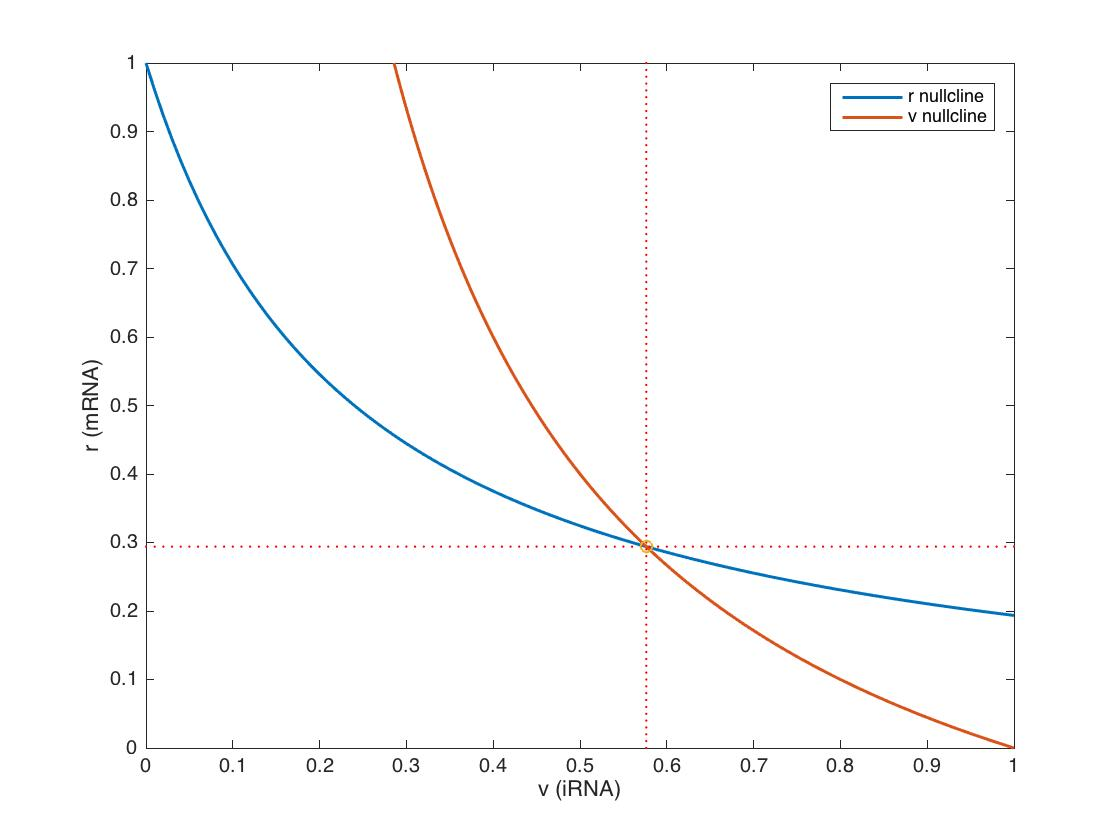
\includegraphics[width=\linewidth]{deterss}
\caption{the phase protrait of the nondimensionalized system derives one real positive steady state calculated based on the nullclines.}
\label{fig:deterss}
\end{figure}

%As shown in Figure \ref{fig:deterdyn}

\begin{figure}[ht]
\centering
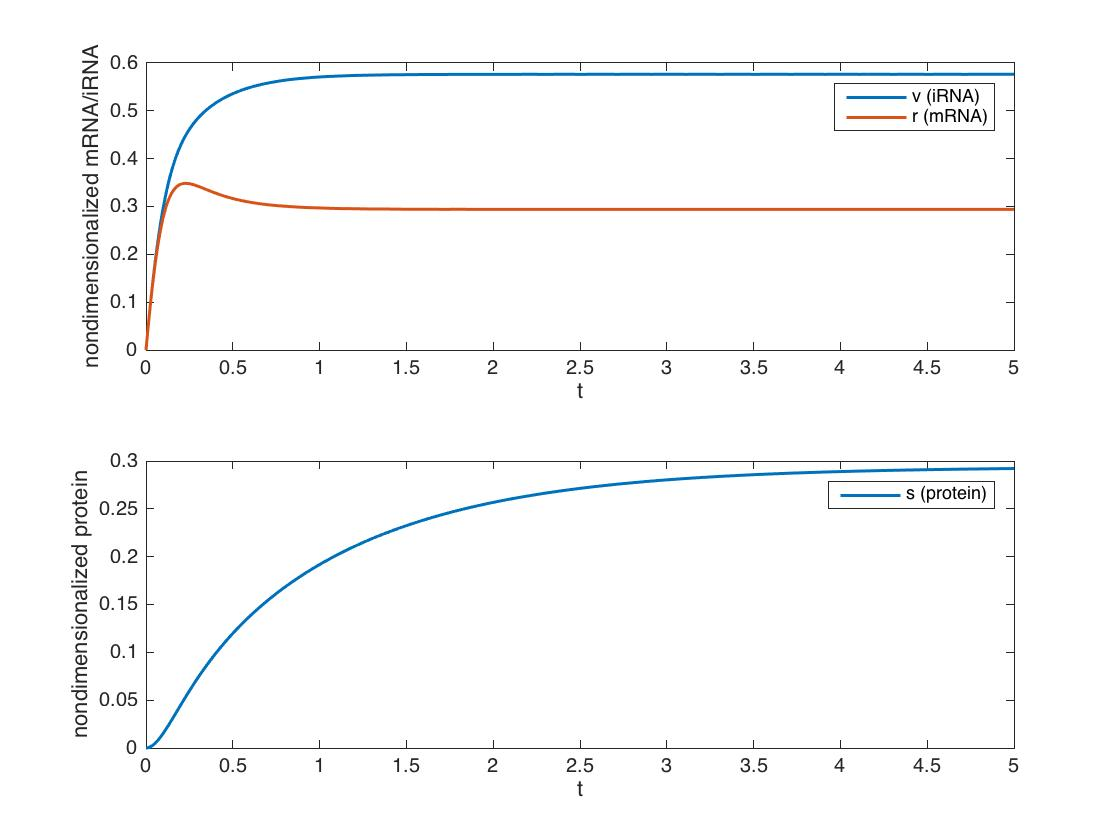
\includegraphics[width=\linewidth]{deterdyn}
\caption{the determinisitic dynamics of the system of mRNA, iRNA and protein.}
\label{fig:deterdyn}
\end{figure}

\subsection*{Chemical Master Equation and Single-Molecule Kinetics}


The chemical master equation of this system can be specified as:
\begin{equation}
\begin{aligned}
\frac{dP(m,n,p)}{dt} = K_2P(m, n - 1, p) + K_1P(m - 1, n, p) + mK_3P(m, n, p - 1) \\ + [(n + 1)\gamma_1 + m(n + 1)H]P(m, n + 1, p)  \\ + (p + 1)\gamma_3P(m, n, p + 1) + [(m + 1)\gamma_1 + (m + 1)nH]P(m + 1, n, p)\\ - P(m, n, p)(K_2 + P\gamma_3 + K_1 + mK_3 + n\gamma_1 + mnH + m\gamma_1 + mnH)
\end{aligned}
\end{equation}
\begin{equation}
\begin{aligned}
\frac{dP(0,n,p)}{dt} = K_2P(0, n - 1, p) +  (n + 1)\gamma_1P(0, n + 1, p) + (p + 1)\gamma_3P(0, n, p + 1) \\+ (\gamma_1 + nH)P(1, n, p) - P(0, n, p)(K_2 + P\gamma_3 + K_1 + n\gamma_1)
\end{aligned}
\end{equation}
\begin{equation}
\begin{aligned}
\frac{dP(m,0,p)}{dt} = K_1P(m - 1, 0, p) + mK_3P(m, 0, p - 1) + [\gamma_1 + mH]P(m, 1, p) \\+ (p + 1)\gamma_3P(m, 0, p + 1) + (m + 1)\gamma_1P(m + 1, 0, p) \\- P(m, 0, p)(K_2 + P\gamma_3 + K_1 + mK_3 + m\gamma_1)
\end{aligned}
\end{equation}
\begin{equation}
\begin{aligned}
\frac{dP(m,n,0)}{dt} = K_2P(m, n - 1, -) + K_1P(m - 1, n, 0)+ [(n + 1)\gamma_1 + m(n + 1)H]P(m, n + 1, 0)\\ + \gamma_3P(m, n, 1) + [(m + 1)\gamma_1 + (m + 1)nH]P(m + 1, n, 0) \\- P(m, n, 0)(K_2 + P\gamma_3 + K_1 + mK_3 \\+ n\gamma_1 + mnH + m\gamma_1 + mnH)
\end{aligned}
\end{equation}

As shown in Figure \ref{fig:cme}, the transition diagram is in 3 dimensions, in the number of iRNA molecule, mRNA molecule, and protein molecule. Different from the stochastic system of transcription factor, the iRNA and mRNA axes are independent of protein axis.

\begin{figure}[ht]
\centering
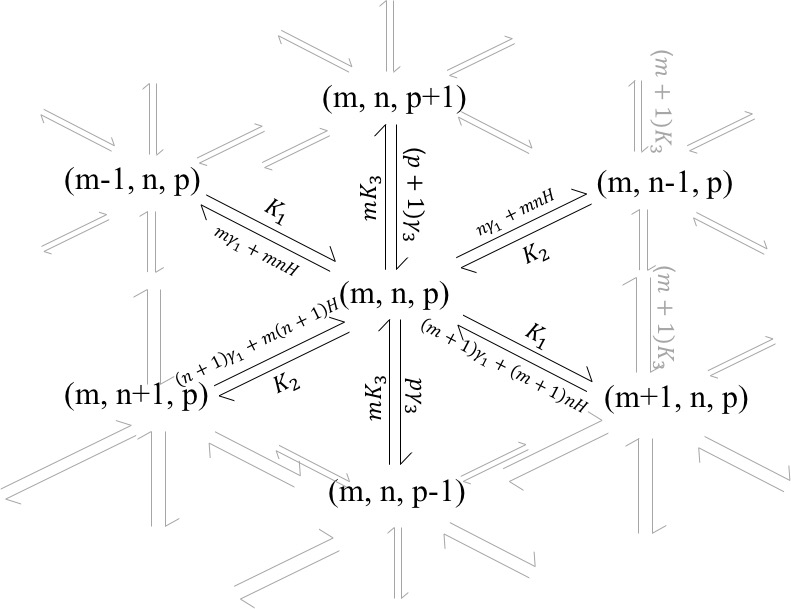
\includegraphics[width=\linewidth]{cme}
\caption{a discrete schematic illustrating the Markovian kinetics of a single molecule of iRNA, mRNA, or protein with conformational fluctuations.}
\label{fig:cme}
\end{figure}

Based on the specified chemical master equation, the stochastic dynamics of the system is shown in Figure \ref{fig:stochsim}, starting from (0, 0, 0).

\begin{figure}[ht]
\centering
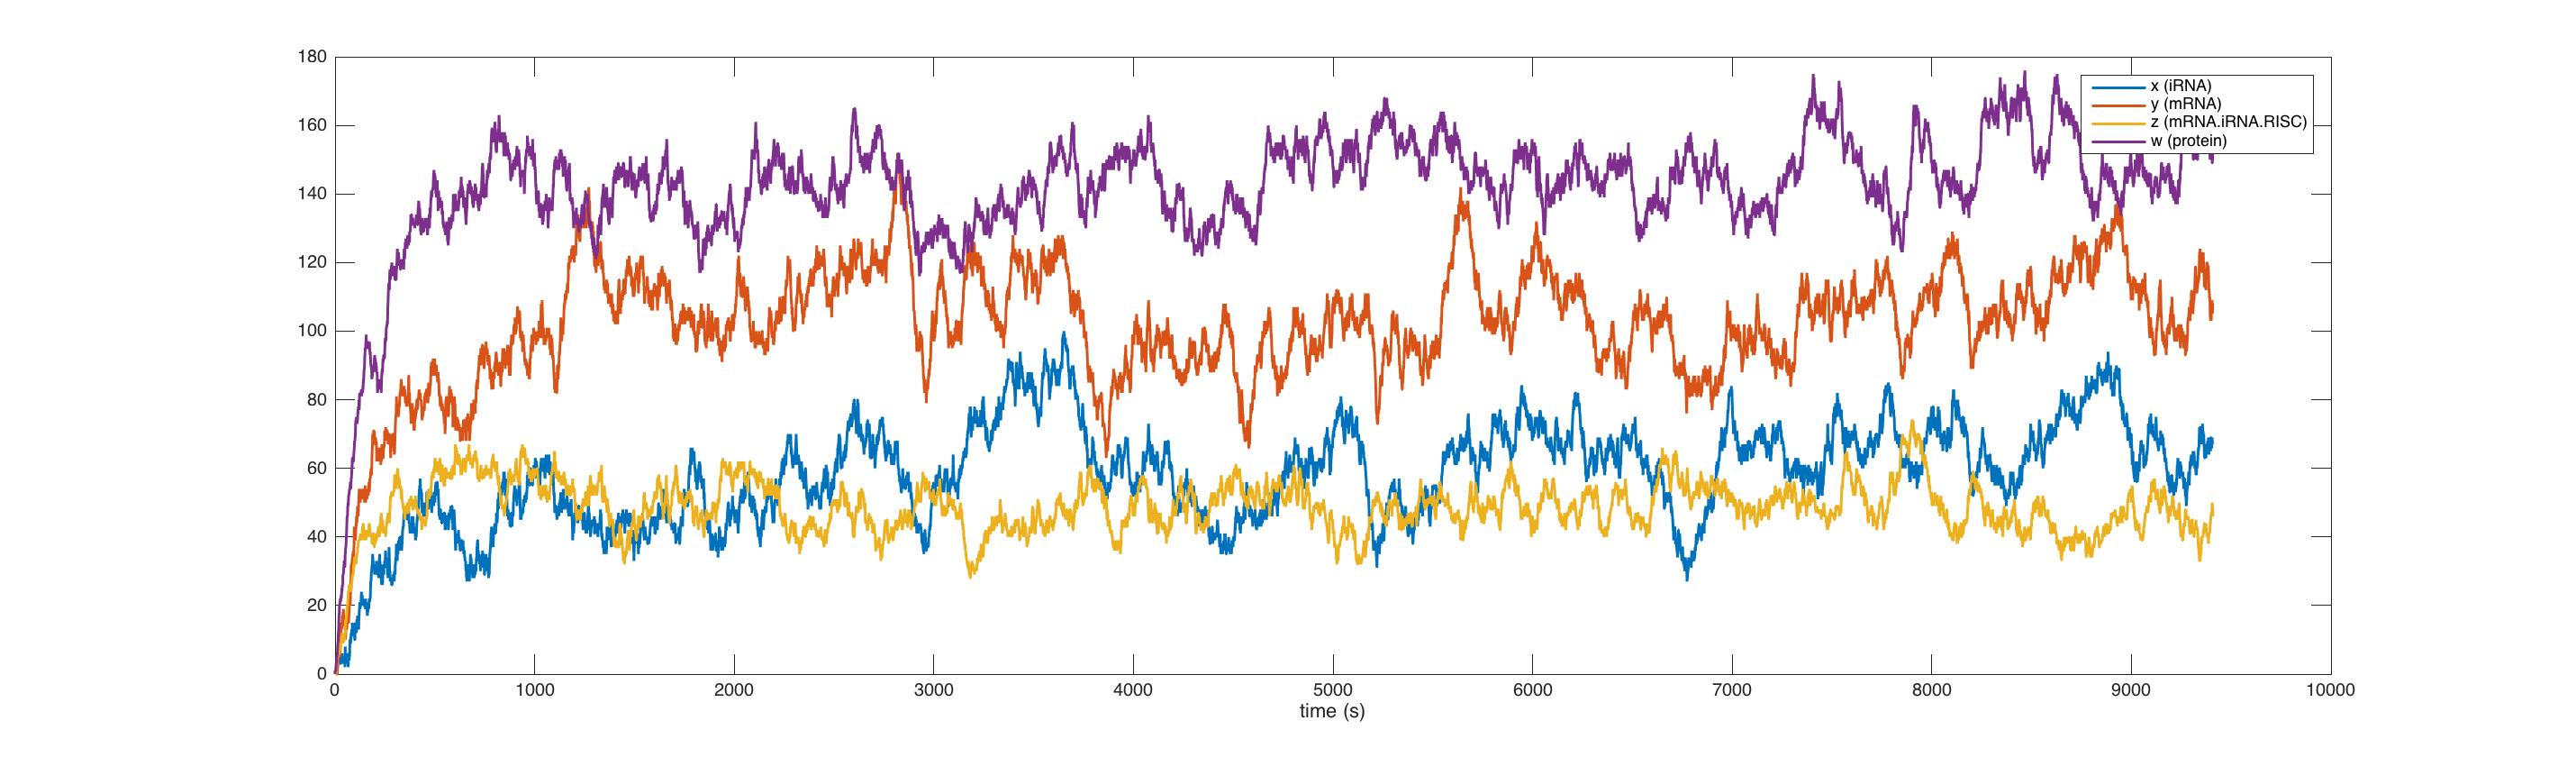
\includegraphics[width=\linewidth]{stochsim}
\caption{the stochastic dynamics of the system of mRNA, iRNA and protein.}
\label{fig:stochsim}
\end{figure}

\section*{Discussion}

As shown from the exploration a



\bibliography{sample}

\noindent LaTeX formats citations and references automatically using the bibliography records in your .bib file, which you can edit via the project menu. Use the cite command for an inline citation, e.g.  \cite{Figueredo:2009dg}.

\section*{Acknowledgements}

Thank Prof. Qian for giving us insightful lectures about the mathematical theories of cellular dynamic and the exciting field of mathematical biology. Thank him for always setting challenging questions for me to explore! Thank my friends in AMATH 531 who come along with me in great energy! Thank University of Washington for giving me the platform to scientifically explore problems and subjects! I will continue the voyage of exploring the infinite realm of mathematical and systems biology in my academic career fearlessly.

\section*{Additional information}

For supporting MATLAB Codes, please refer to Supplementary Information Attached. All code for the reproduction of the reported results can be downloaded from my \href{https://github.com/doerlbh/RNAi_CME_Dynamics}{GitHub Repository}.

\end{document}